\documentclass[]{standalone}
%\usepackage{mathptmx}
%\renewcommand{\familydefault}{\rmdefault}
\usepackage[T1]{fontenc}
\usepackage[latin9]{inputenc}
\usepackage{siunitx}
\usepackage{array}
\usepackage{amsmath}
\usepackage{ifthen}
\usepackage{pgfplots}
\pgfplotsset{compat=1.14}
\usepackage{titling, graphicx}
\usepackage{tikz}
\usepackage{upgreek}
\usepackage{amsmath,amsthm}
\usepackage{strtikz}
\usetikzlibrary{shapes,arrows.meta,intersections,graphs,graphs.standard}
\usetikzlibrary{bending, math,fit, patterns, patterns.meta}
\usetikzlibrary{calc,intersections,through,backgrounds,decorations.pathmorphing}
%\usetikzlibrary{fpu}
%\usepackage{pgfmath}


\begin{document}


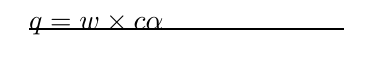
\begin{tikzpicture}
\draw [line width=1](0, 0) -- ++(4cm,0cm);
\frametrapezoidalload[startx = 0cm,
starty = 0cm,
endx = 4cm,
endy = 0cm,
number of arrows = 15,
print first arrow = 1,
print last arrow = 1,
height of arrows left= 0.4cm,
height of arrows mid = 0.5cm,
height of arrows right= 0.4cm,
mid ratio left = 0.1,
mid ratio right = 0.1,
load angle=10,
space = 2pt,
start ratio = 0.05,
end ratio = 0.05,
mid load text = ${q=w \times c}$,
left load text = $$,
right load text = $$,
text color=black,
mid text shiftx=0pt,
mid text shifty=-2pt,
left text shiftx=0pt,
left text shifty=0pt,
right text shiftx=0pt,
right text shifty=0pt,
arrow length=5pt,
arrow width=3pt,
arrow scale=1,
arrow line thickness=1pt,
arrow color=blue!75,
draw angle = 0,
angle arrow number = 10,
angle line thickness = 0.5pt,
angle length = 2cm,
angle space = 0.1cm,
angle location = 2cm,
angle text = $\alpha$,
angle text xshift = 0.0cm,
angle text yshift = 0.0cm,
draw ninety sign=0,
ninety sign dimension=0.2cm,
ninety sign factor=4,]
%$\SI{10}{\kilo\newton/\meter}$


\end{tikzpicture}




\end{document}
